\documentclass[12pt]{article}
\usepackage[english]{babel}
\usepackage{natbib}
\usepackage{url}
\usepackage[utf8x]{inputenc}
\usepackage{amsmath}
\usepackage{graphicx}
\usepackage{hyperref}
\graphicspath{{images/}}
\usepackage{parskip}
\usepackage{fancyhdr}
\usepackage{vmargin}
\setmarginsrb{3 cm}{2.5 cm}{3 cm}{2.5 cm}{1 cm}{1.5 cm}{1 cm}{1.5 cm}
\usepackage{hyperref}

\title{BeerEX: the Beer EXpert system}
\author{Donato Meoli}
\date{September 11, 2019}

\makeatletter
\let\thetitle\@title
\let\theauthor\@author
\let\thedate\@date
\makeatother

\pagestyle{fancy}
\fancyhf{}
\rhead{\theauthor}
\lhead{\thetitle}
\cfoot{\thepage}

\begin{document}

\begin{titlepage}
	\centering
    \vspace*{0.5 cm}
    
\includegraphics[scale = 0.5]{img/unipi.png}\\[1.0 cm]
    \textsc{\LARGE University of Pisa}\\[0.5 cm]
    \textsc{\Large Department of Computer Science}\\[1.5 cm]
	\textsc{\large Artificial Intelligence Fundamentals}\\[0.5 cm]
	\rule{\linewidth}{0.2 mm} \\[0.4 cm]
	{ \huge \bfseries \thetitle}\\
	\rule{\linewidth}{0.2 mm} \\[1.5 cm]
	\centering \textsc{\large \emph{Author:}}\\[0.5 cm]
	\begin{minipage}{0.4\textwidth}
		\begin{center} \large
			\textbf{\theauthor}
		\end{center}
		\end{minipage}~
		\begin{minipage}{0.4\textwidth}
	\end{minipage}\\[2 cm]
	{\large \thedate}\\[2 cm]
	\vfill
\end{titlepage}

\tableofcontents
\pagebreak

\section{Context \& Background}

\subsection{The Context of BeerEX}
The expert system \textit{BeerEX} - \textit{Beer EXpert system} - was designed to suggest a beer to drink according to taste and meal. The choice of building such a system was dictated by the vastness of the product market and by the lack of information that is usually found in consumers. The system is essentially useful for people who want to taste appropriate beers and would like to know in real time the most suitable beer based on their tastes and/or based on the meals they are going to consume. Through simple questions the system recognizes the tastes of the user returning also indications on how each question helps to arrive at the solution of the problem. BeerEX works with a dataset of beer styles, therefore a limited domain on which the rules have greater inferential power, thus not providing for recommending any beer on the market, but rather the style to which it is associated. Each style of beer has characteristics about the \textit{flavor}, \textit{color}, \textit{alcohol} content and \textit{carbonation}, etc.: all aspects on which the user will be able to express their preferences. The system uses the dataset made available by the American association \href{https://www.craftbeer.com}{CraftBeer}. 

At the beginning of 2016, in the United States alone, there are more than 5,000 breweries responsible for the various beer brands, around 150 different beer styles and over 20,000 brands. Furthermore, the market is expanding more and more: according to the estimates of the \href{https://www.brewersassociation.org}{Brewers Association} there was an increase of about 800 breweries compared to the previous year (always in the US market), for a total of 129,000 employees in the sector and an economic impact of around 56 billion dollars.

\begin{figure}[h]
\centering
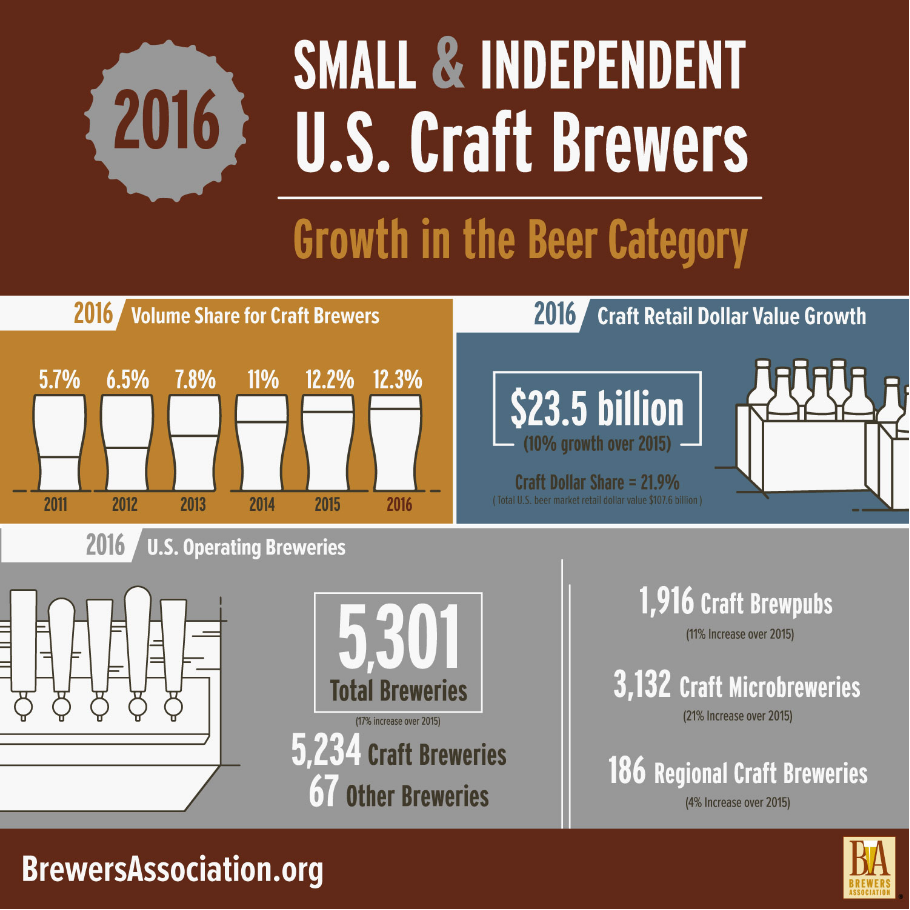
\includegraphics[scale = 0.4]{img/brewers.png}
\caption{Operative breweries in the United States in 2016}
\end{figure}

\subsection{Why an Expert System}
Conventional programming languages ​​are designed for procedural data manipulation. Humans, however, often solve complex problems using very abstract symbolic approaches that cannot be implemented with conventional languages. One of the research results in the area of ​​Artificial Intelligence has been the development of techniques that allow the modeling of information at higher levels of abstraction. These techniques are incorporated into logical languages ​​or tools that allows to build programs that closely resemble human logic in their implementation and are therefore easier to develop and maintain. Some of these tools, which emulate human skills in well-defined problem domains, are called expert systems. 

Rules-based programming is one of the most commonly used techniques for developing expert systems. In this programming paradigm, \textit{rules} and \text{facts} are used to represent the expert's knowldge and then, the inference engine, equipped with a powerful pattern matching algorithm, called Rete, will verify the matching of a rule through his left-hand side in accordance with the state of the world or the working memory.

\begin{figure}[h]
\centering
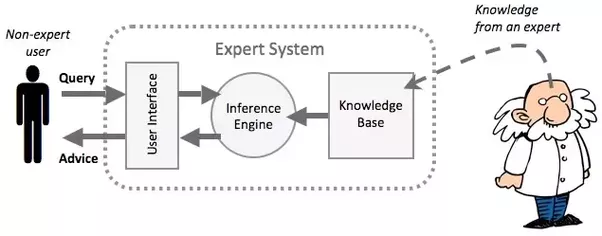
\includegraphics[scale = 0.6]{img/arch.png}
\caption{Architecture of an Expert System}
\end{figure}

\section{Description of the System}

\subsection{Modular Organization}

The system is divided into several modules:
\begin{itemize}
\item \textbf{beer-questions.clp}: file containing the questions that can be asked to the user;
\item \textbf{beer-knowledge.clp}: file containing the knowledge of the expert as rules;
\item \textbf{beer-styles.fct}: beer styles dataset;
\item \textbf{beerex.clp}: main file containing the template definitions and import all the previous ones.
\end{itemize}

\subsection{Reasoning under Uncertainty}

The system's knowledge brings with it a degree of uncertainty: in general, in expert systems, a subjective probability formulated by experts is used. A statistical theory of evidence is provided by the Bayes reasoning which, being computationally intractable, was used to develop \textit{certainty factors}, ie relatively informal mechanisms to quantify the levels of trust to be assigned to a given conclusion based on proven facts. In BeerEX it is possible that two or more rules can draw conclusions about facts asserted in the working memory with different certainty factors. In order to calculate the certainty factor, BeerEX combines these weights using the following formula to obtain a single certainty factor:

\[
   CF(X,Y) =
   \begin{cases}
      X+Y-XY & se X,Y > 0 \\
      X+Y+XY & se X,Y < 0 \\
      \frac{X+Y}{1-min(|X|,|Y|)} & altrimenti
   \end{cases}
\]

where X and Y are the certainty factors included in the interval [-1; 1], where -1 indicates the maximum degree of distrust with which the fact is asserted, 1 indicates the maximum degree of trust with which the fact is asserted, while $\forall$ n $\in$ (-1; 1) all the degrees of intermediate truths.

\subsection{User Scenario}
The system is able to recognize the user scenario through some initial random and more generic questions about \textit{sex} (to determine how strong the recommended beer is in terms of alcohol and taste), the \textit{age} (useful for determining how strong in terms of alcohol and taste will be the recommended beer), the current \textit{season} (weather conditions affect our perceptions and needs), the \textit{frequency} with which the user is usually \textit{drinking beer} (useful for being able to propose more particular beer styles in case the user is a frequent beer drinker), if he \textit{smokes} (the taste of tobacco could alter the taste of beer or beers with a lot of flavor intense could bind particularly well with the taste of tobacco), etc.

After having at least framed the type of user in front of him, the system will ask more specific questions about preferences about the \textit{flavor}, \textit{color}, \textit{alcohol} content, \textit{carbonation}, etc. and, finally, in the event that the user is about to eat, a series of increasingly specific questions about the meal (main component, type, type of cooking, etc.).

\subsection{Use Aids}
The system lends itself to be suitable for different degrees of user experience about the beer domain by providing two possible commands:
\begin{itemize}
\item \textbf{help}: this command allows the user to show an explanation of the question for a better understanding of the same;
\item \textbf{why}: this command allows the user to show a reason why the question was asked.
\end{itemize}

\subsection{Results, Explanation \& Retraction}

One of the greatest potentials of an expert system compared to other modern intelligent systems lies in being able to explain the motivation of the choices made, therefore, at the end of the execution the system will return the most appropriate beers selected on the basis of the answers received and of the inference made with a relative explanation.

Moreover, since it is a \textit{TMS} - \textit{Truth Maintenance System} - at the end as well as in every moment of the execution it is possible to go back to be able to change the answer to a question and retract what was asserted from that moment on, bringing the system back into a consistent state.

\newpage
\section{Extensions}

\subsection{Telegram ChatBot}
Assuming that the real utility of the system can be subsidized not in front of a computer but during daily outings in pubs and restaurants and being CLIPS a portable and embeddable tool, it was thought to make it usable beyond a CLI environment, allowing it to interact through a Telegram chatbot simulating a conversation with the expert, obviously completely leaving the logical part of the system unaltered in CLIPS language.

\begin{figure}[h]
\centering
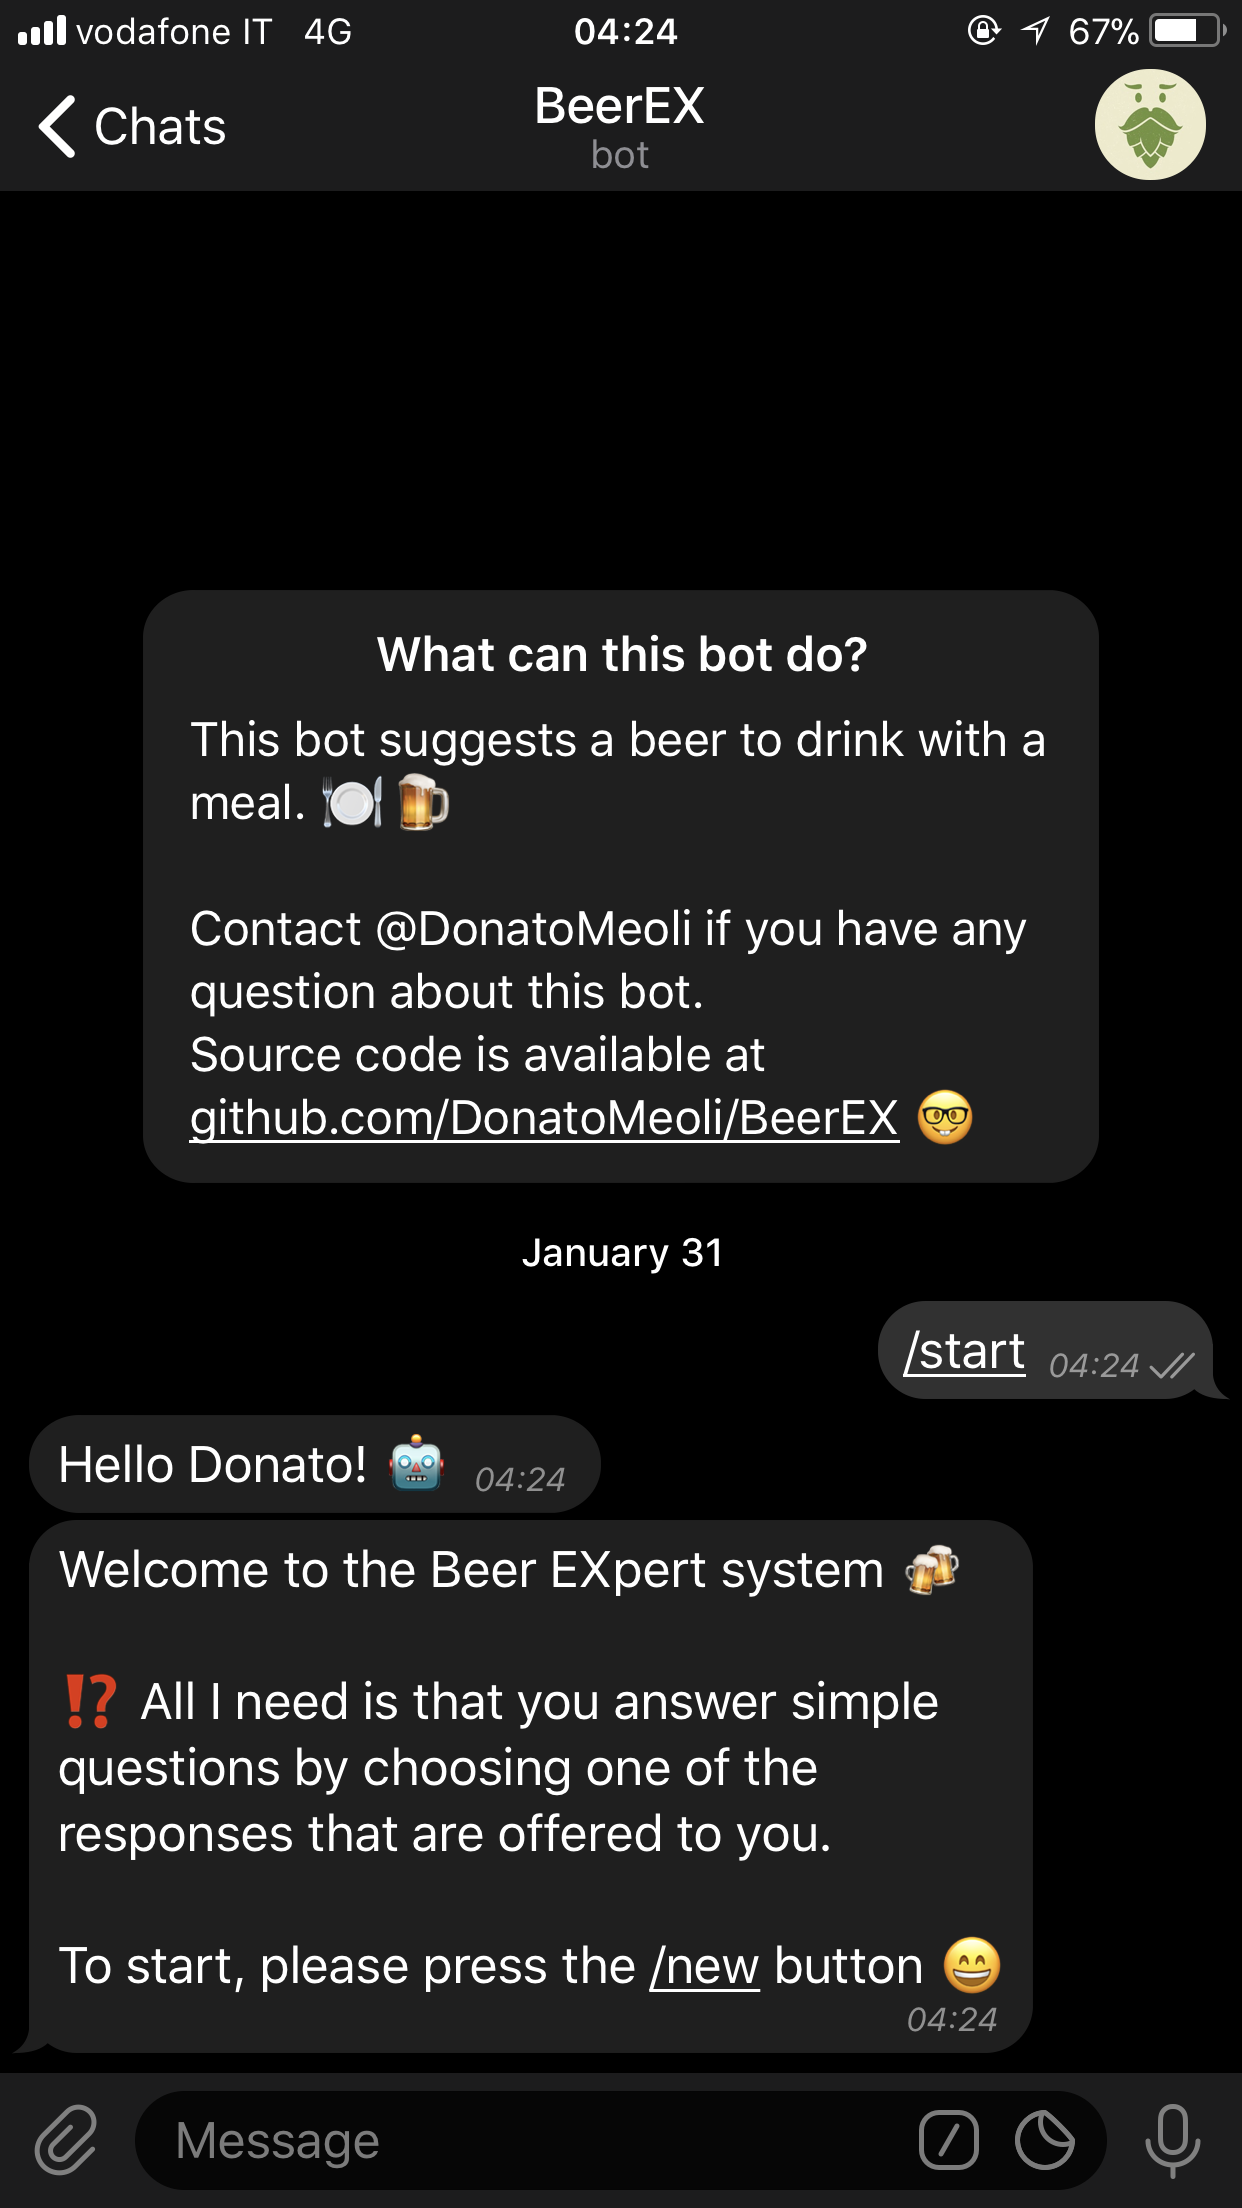
\includegraphics[scale=0.13]{img/bot1.png}\quad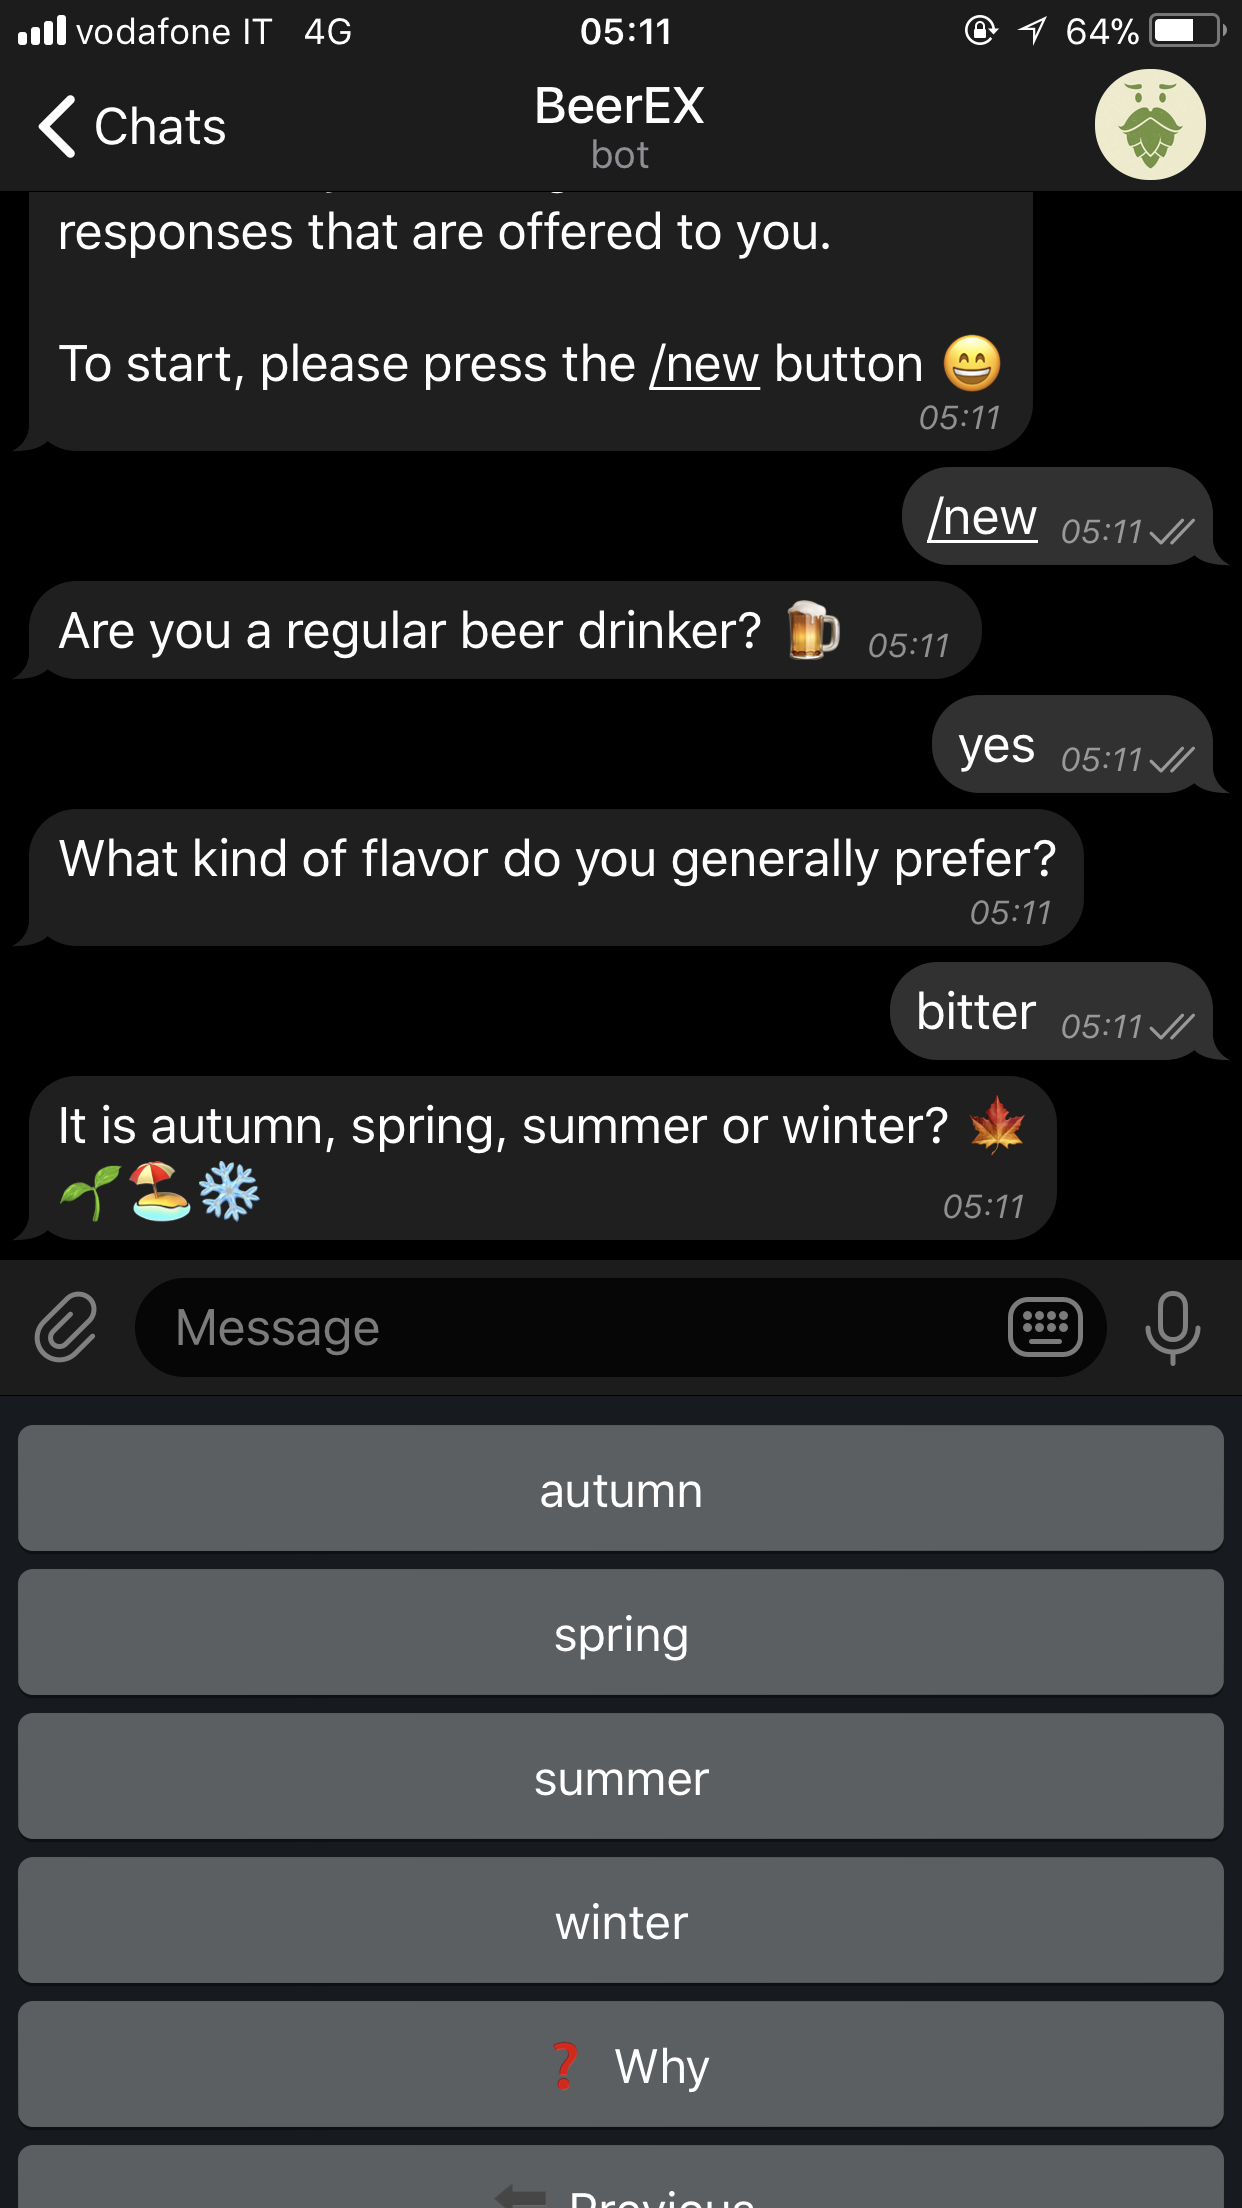
\includegraphics[scale=0.13]{img/bot2.png}
\caption{The chatbot running}
\end{figure}

\begin{figure}[h]
\centering
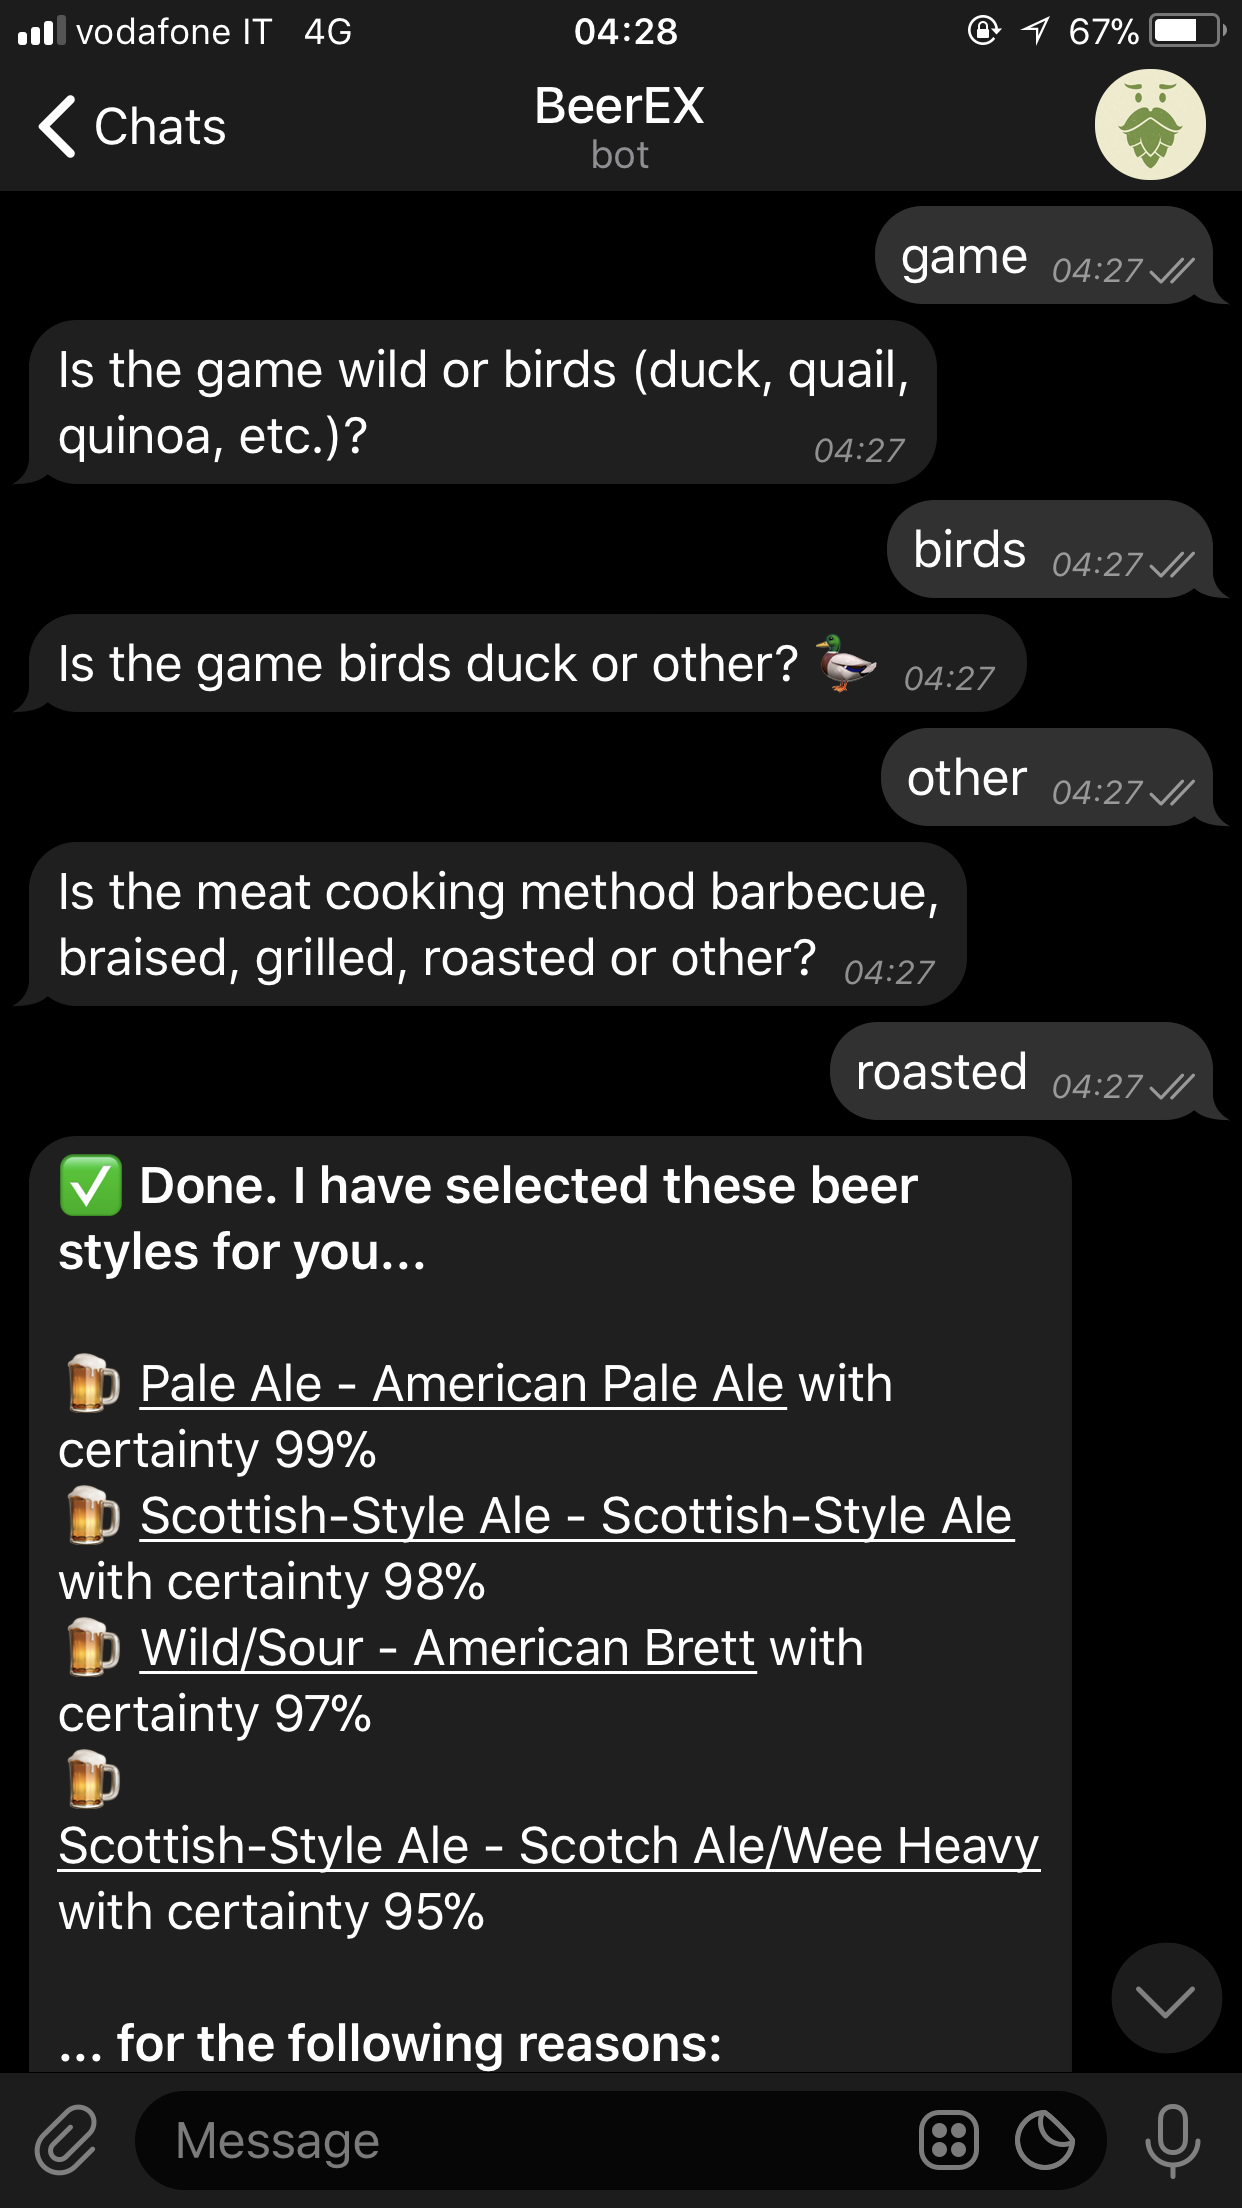
\includegraphics[scale=0.13]{img/bot3.png}\quad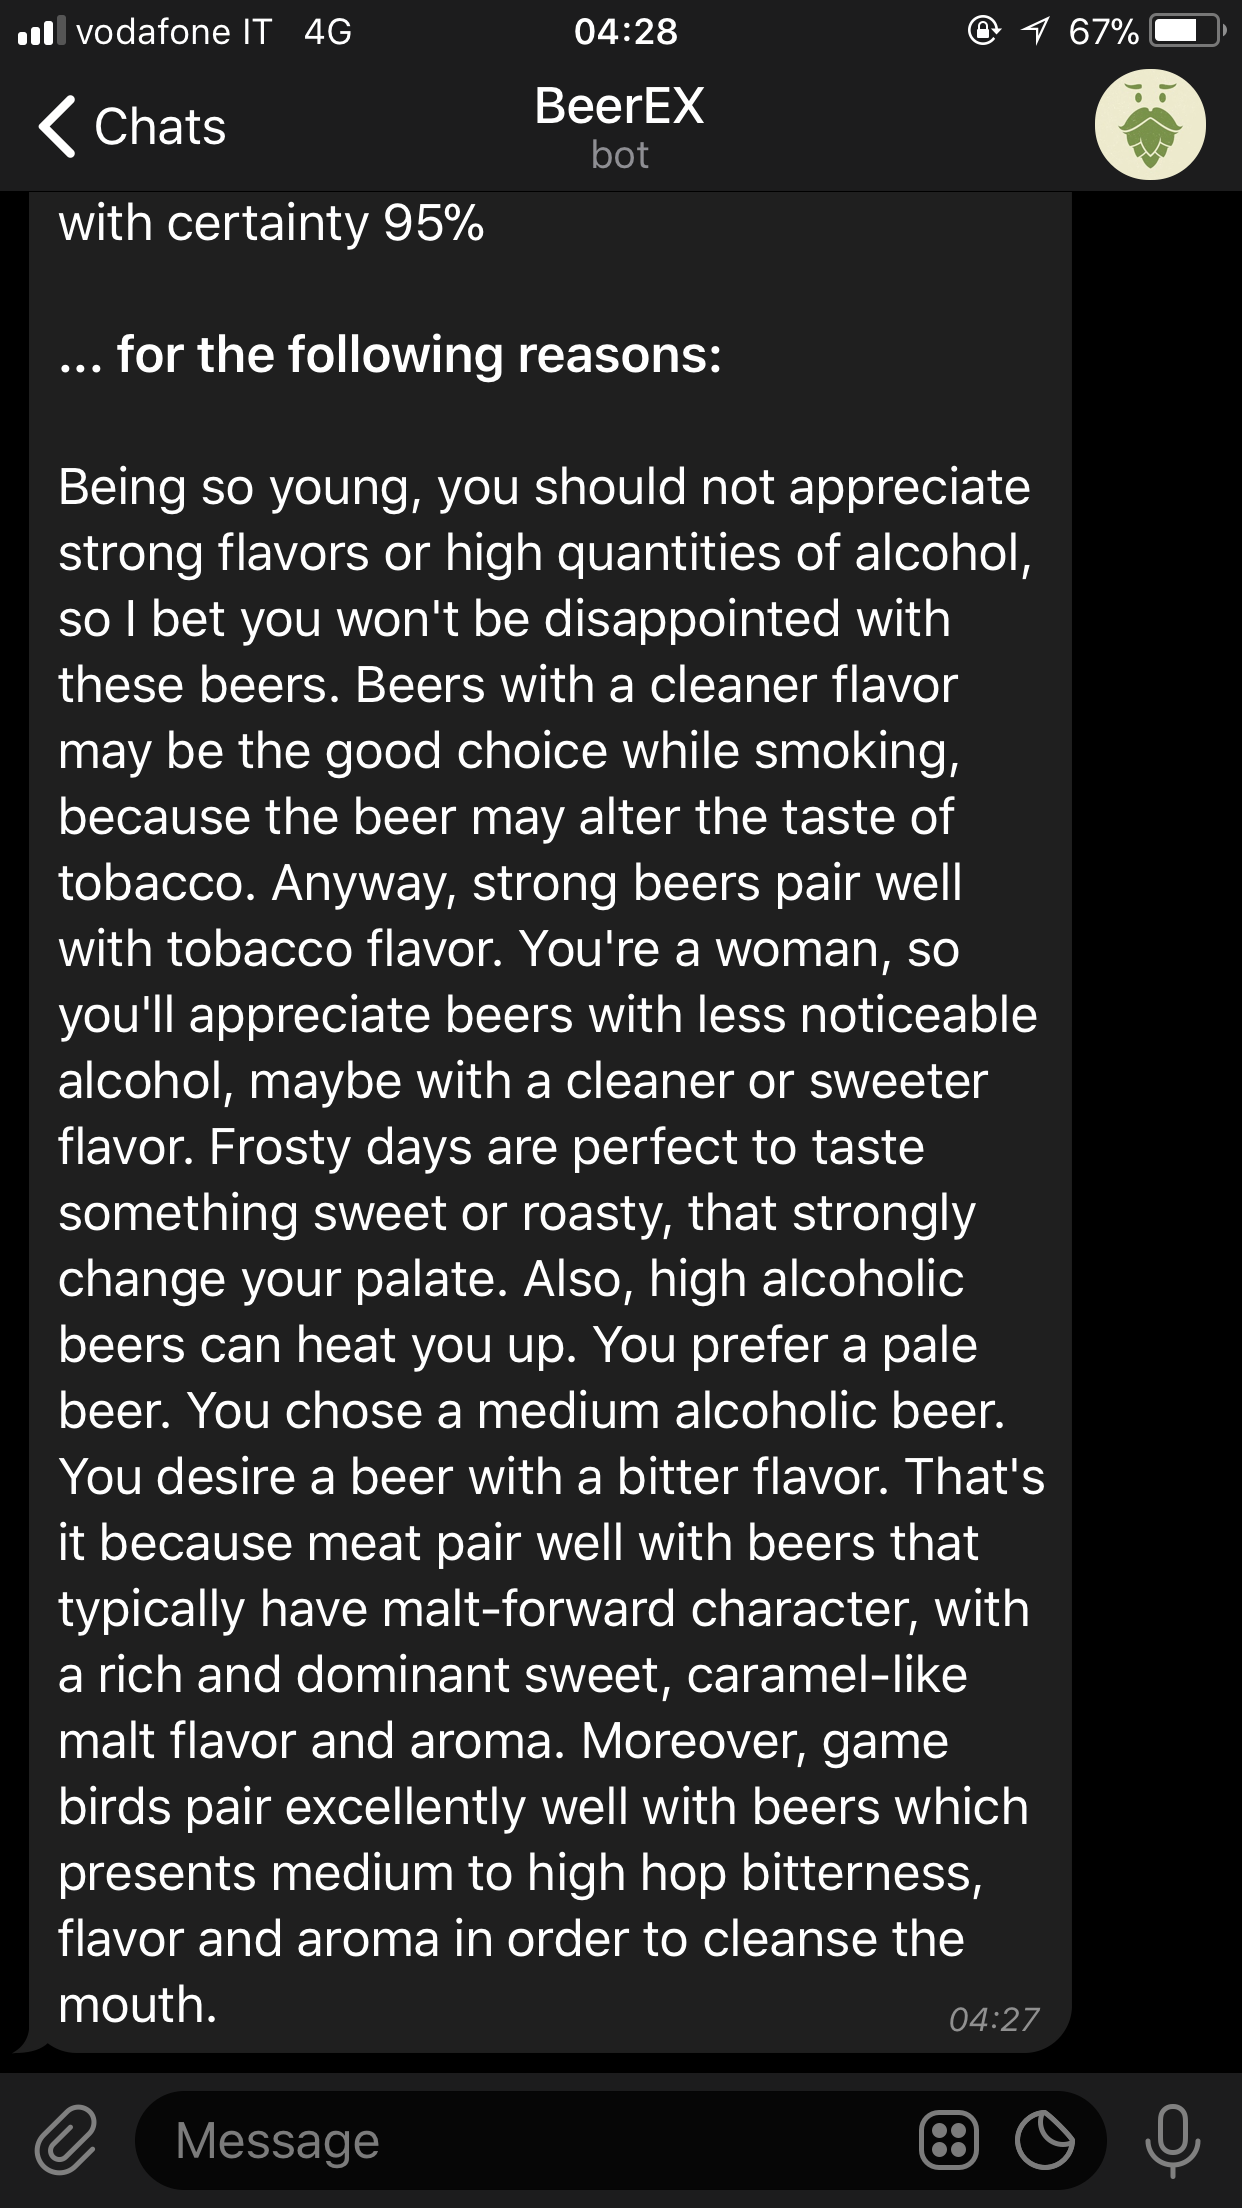
\includegraphics[scale=0.13]{img/bot4.png}
\caption{The chatbot results and relative reasons}
\end{figure}

\newpage
\bibliographystyle{plain}
\bibliography{biblist}

\end{document}
